\documentclass[letterpaper,final,12pt,reqno]{amsart}

\usepackage[total={6.3in,9.2in},top=1.1in,left=1.1in]{geometry}

\usepackage{times,bm,bbm,empheq,fancyvrb,graphicx}
\usepackage[dvipsnames]{xcolor}
\usepackage{tikz}
\usetikzlibrary{decorations.pathreplacing}

\usepackage[kw]{pseudo}
\pseudoset{left-margin=15mm,topsep=5mm,idfont=\texttt}

% hyperref should be the last package we load
\usepackage[pdftex,
colorlinks=true,
plainpages=false, % only if colorlinks=true
linkcolor=blue,   % ...
citecolor=Red,    % ...
urlcolor=black    % ...
]{hyperref}

\renewcommand{\baselinestretch}{1.05}

\newtheorem{lemma}{Lemma}

\newcommand{\Matlab}{\textsc{Matlab}\xspace}
\newcommand{\eps}{\epsilon}
\newcommand{\RR}{\mathbb{R}}

\newcommand{\grad}{\nabla}
\newcommand{\Div}{\nabla\cdot}
\newcommand{\trace}{\operatorname{tr}}

\newcommand{\hbn}{\hat{\mathbf{n}}}

\newcommand{\bb}{\mathbf{b}}
\newcommand{\bbf}{\mathbf{f}}
\newcommand{\bg}{\mathbf{g}}
\newcommand{\bn}{\mathbf{n}}
\newcommand{\bu}{\mathbf{u}}
\newcommand{\bv}{\mathbf{v}}
\newcommand{\bw}{\mathbf{w}}
\newcommand{\bx}{\mathbf{x}}

\newcommand{\bV}{\mathbf{V}}
\newcommand{\bX}{\mathbf{X}}

\newcommand{\bxi}{\bm{\xi}}

\newcommand{\bzero}{\bm{0}}

\newcommand{\rhoi}{\rho_{\text{i}}}

\newcommand{\ip}[2]{\left<#1,#2\right>}


\begin{document}
\title[Geometric multigrid for glacier modeling]{Geometric multigrid for glacier modeling: \\ A user's guide}

\author{Ed Bueler}

\begin{abstract} FIXME: two principles in introduction: mass conservation complementarity, solver optimality.  four examples in sections \ref{sec:subspace}--\ref{sec:stokes}: poisson equation from subspace decomp point of view, obstacle problem by subset decomposition, monotone multigrid for implicitly-evolving SIA geometry, Schur-complement and Vanka Newton-multigrid for fixed-geometry Glen-Stokes
\end{abstract}

\maketitle

\tableofcontents

\thispagestyle{empty}
\bigskip

\section{Introduction} \label{sec:intro}

The construction of effective numerical glacier and ice sheet models is challenging for two fundamental reasons.  First is the complexity of the equations and boundary conditions.  Indeed, the physics of glaciers is nonlinear, nontrivially-coupled, and subject to imperfectly-understood boundary processes, such as at contact with ocean water.  The coupling is critical in the sense that mass, momentum, and energy conservation interact in ways which are relevant to glaciological modeling goals, such as when basal sliding, and thus ice velocity, is only determined though a simultaneous momentum and energy solution.  Second, the geometry of glaciers and ice sheets is complex, and in particular the fastest-flowing parts of ice sheets are often located at the geometrically-nontrivial lateral boundary where fjord-like bed geometry is also common.  Numerical models therefore need to perform expensive fine-mesh calculations, so as to accomodate the complicated, changing boundary geometry, while solving relatively-complicated multiphysics equations.

On the other hand, since the 1980s researchers in numerial methods have developed multigrid methods to solve partial differential equations like those which describe the ice fluid in glaciers.   For simpler problems like scalar elliptic equations and the linear Stokes system, especially on domains which have a simpler geometry, these methods are now in routine use \cite{Briggsetal2000,Bueler2021,Trottenbergetal2001}.

FIXME perspectives \emph{not} found here: convergence of GMG (or much detail for application to linear problems); assumptions like ``SPD'' specific to constrained \emph{optimization} as opposed to VI/NCP viewpoint


\section{From subspace decomposition to multigrid (Poisson equation)} \label{sec:subspace}

To introduce multigrid methods we will first demonstrate how to solve a simple ordinary differential equation (ODE), namely the Poisson problem
\begin{equation}
- u''(x) = f(x) \quad \text{on} \quad 0 \le x \le 1, \label{eq:poisson}
\end{equation}
with boundary conditions $u(0)=u(1)=0$.  Over the course of this and the next two sections, this simple equation will ``evolve'' into a realistic model for glacier geometry.  Along the way we will develop the multigrid ideas.

Our numerical approximation of \eqref{eq:poisson} uses an unequally-spaced mesh of $m$ interior \emph{nodes} (points) $x_p$ as shown in Figure \ref{fig:finehats}.  The open subintervals between the nodes are the \emph{elements}.  The numerical solution $u^h(x)$ will be constructed as a linear combination of the piecewise-linear hat functions $\psi_p(x)$, shown in Figure \ref{fig:finehats}, one for each interior node:
\begin{equation}
u^h(x) = \sum_{p=1}^m u_p \psi_p(x). \label{eq:trialsolution}
\end{equation}
Each hat function is defined on all of $[0,1]$ by $\psi_p(x_q) = \delta_{pq}$ and by being linear between the nodes and continuous.  In fact, $\{\psi_p(x)\}_{p=1}^m$ is a basis of the space $\mathcal{V}^h$ of continuous, piecewise-linear functions, and it is a \emph{nodal basis} in the sense that the coefficients are the values of the function: $u_p=u^h(x_p)$.  Note that the derivative of $u^h(x)$ is defined on the elements, but not generally at the nodes.

\begin{figure}
\includegraphics[width=0.75\textwidth]{figs/finehats.pdf}
\caption{Hat functions $\psi_p(x)$ at the interior points $x_p$ form a basis for the vector space of piecewise-linear functions  with zero boundary values $\mathcal{V}^h$.}
\label{fig:finehats}
\end{figure}

Having represented the solution, if we want to actually solve the problem then we must adjust the coefficients $u_p$ to their correct values.  In a program these coefficients are formed into a column vector, denoted $\bu=\{u_p\}$ in $\RR^m$.  We may directly use equation \eqref{eq:poisson} and a finite difference (FD) method \cite{LeVeque2007} to construct a linear system to determine $\bu$.  However, our applications of multigrid ideas to glacier problems will be much clearer if we instead adopt a finite element (FE) approach based on re-phrasing \eqref{eq:poisson} in \emph{weak form} using integrals.  (Accessible introductions to FE methods are in \cite{Bueler2021,Elmanetal2014,Johnson2009}.)  Note that once we state the weak form, next, then the original equation \eqref{eq:poisson} will be called the \emph{strong form}.

The weak form of \eqref{eq:poisson} arises by multiplying both sides of the equation by a \emph{test function} and integrating by parts so that only first derivatives remain.  Without committing to any mathematical detail, we suppose the exact, continuum solution $u(x)$ comes from a vector space $\mathcal{H}$ of functions which are smooth enough to allow the computations which follow and which have value zero at $x=0$ and $x=1$.  Choosing a test function $v(x)$ also from $\mathcal{H}$, by multiplying and integrating by parts, and by using $v(0)=v(1)=0$, we find that equation \eqref{eq:poisson} implies
\begin{equation}
\int_0^1 u'(x) v'(x)\,dx = \int_0^1 f(x) v(x)\, dx.  \label{eq:weakpoissonearly}
\end{equation}
We write equation \eqref{eq:weakpoissonearly} more compactly as
\begin{equation}
  a(u,v) = \ip{f}{v} \label{eq:weakpoisson}
\end{equation}
where each side is defined exactly as the corresponding side in \eqref{eq:weakpoissonearly}.  (The reasons for this notational simplification will become clear as we describe multigrid ideas and algorithms.)  For $u,v$ in $\mathcal{H}$, the left side $a(u,v)$ is linear in each argument (\emph{bilinear}) while the right side defines a \emph{linear functional} $v\mapsto \ip{f}{v}$.

One may substitute the \emph{trial} formula \eqref{eq:trialsolution} for $u^h$ into \eqref{eq:weakpoisson} to derive a linear system
\begin{equation}
A \bu = \bbf, \label{eq:linearsystem}
\end{equation}
where $A$ is an $m\times m$ matrix and $\bbf$ is in $\RR^m$.  Each equation in the linear system is constructed by using a hat function as a test function.  That is, substitution of $v=\psi_p$ into \eqref{eq:weakpoisson} gives the $p$th equation in FE system \eqref{eq:linearsystem}.  The symmetric matrix $A$, which is positive definite for this Poisson equation \cite{Elmanetal2014}, has entries $a_{pq} = a(\psi_p,\psi_q)$.  For the right side one defines $f_p = \ip{f}{\psi_p}$ to form the vector $\bbf = \{f_p\}$.

The most straightforward way to ask a computer to solve the assembled linear system \eqref{eq:linearsystem} would be by a direct method such as Gaussian elimination.  However, in higher-dimensional PDE problems such methods need much more that $O(m)$ operations to solve the system, where $m$ is the number of unknowns.  As noted in the introduction, large-scale applications need optimal $O(m)$ solution methods, or nearly so, thus our focus on multigrid.  Furthermore, after this section all of our problems will be nonlinear, thus no direct (i.e.~finite time) method will be available, and indeed we will generally not assemble matrix objects at all.

On the basis of the above simple FE scheme we can now take the first step to build a \emph{multilevel} or multigrid scheme.  Consider an enlarged set of hat functions:
    $$\underbrace{\psi_1(x),\dots,\psi_m(x)}_{\text{existing fine level}},\underbrace{\psi_{m+1}(x),\dots,\psi_M(x)}_{\text{coarser levels}}$$
The multilevel scheme shown in Figures \ref{fig:finehats} and \ref{fig:coarsehats} includes two coarser levels.  The first coarsening (top of Figure \ref{fig:coarsehats}) comes from by-passing every other node on the fine mesh, and the next coarsening (bottom) does this again.  (On 2D and 3D meshes this manner of constructing coarse-mesh hats is much less straightforward.  It is more common to start from a coarse mesh and refine.)  One may regard the coarsening process as the selection of coarse-mesh nodes, but the hat functions on the coarse level, once identified, contain all the information needed to do coarse-level calculations.

\begin{figure}
\includegraphics[width=0.55\textwidth]{figs/coarsehats.pdf}
\smallskip

\includegraphics[width=0.55\textwidth]{figs/coarsesthats.pdf}
\caption{In our FE method the coarser levels are additional sets of hat functions which spread over a greater distance.}
\label{fig:coarsehats}
\end{figure}

We need notation for the levels.  Suppose that the coarsest is indexed as $k=0$ and the finest as $k=K$, with intermediate levels $k=1,\dots,K-1$.  We index the hat functions by level,
\begin{equation}
  \psi_j^k(x) \quad \text{is the $j$th hat function on the $k$th level},  \label{eq:definepsijk}
\end{equation}
and the interior nodes $x_j^k$ by the same scheme.  There are $m_k$ hats in the $k$th level, thus index $j$ is in the set $\{1,\dots,m_k\}$.  Note the previous notation for the fine mesh has now gained a superscript $K$, thus the hats are $\psi_j^K(x)$ and the nodes are $x_j^K$.  Figures \ref{fig:finehats} and \ref{fig:coarsehats} show a three-level scheme ($K=2$) with a total of $m_2=11$ interior nodes.  There are $m_1=5$ intermediate level nodes and $m_0=2$ coarsest-level nodes.  The fine mesh has $m_2+1=12$ elements, divisible by four, so the above coarsening scheme works.

The $k$th level in our multilevel scheme is really a vector space, namely
\begin{equation}
  \mathcal{V}^k = \operatorname{span}\{\psi_1^k(x),\dots,\psi_{m_k}^k(x)\}.  \label{eq:definevk}
\end{equation}
These hat functions are linearly-independent and form a basis for $\mathcal{V}^k$, thus the dimension of $\mathcal{V}^k$ is $m_k$ and the dimension of the FE solution space $\mathcal{V}^h$, now also denoted $\mathcal{V}^K$, is $m_K$.  In fact these vector spaces are nested, $\mathcal{V}^{k-1} \subset \mathcal{V}^k$, because a coarser-level hat function can be written as a linear combination of next-finer level hats:
\begin{equation}
   \psi_j^{k-1}(x) = \sum_{\ell=1}^{m_k} c_\ell \psi_\ell^k(x). \label{eq:hatcombination}
\end{equation}
The only nonzero coefficients $c_\ell$ are those where the support of $\psi_j^{k-1}(x)$ overlaps with the support of $\psi_\ell^k(x)$.

The multilevel \emph{subspace decomposition} is described by a vector space sum:
\begin{equation}
  \mathcal{V}^h = \mathcal{V}^0 + \mathcal{V}^1 + \dots + \mathcal{V}^K. \label{eq:subspacedecomposition}
\end{equation}
This will be useful even though the final term $\mathcal{V}^K$ is actually equal to the whole space $\mathcal{V}^h$.  Equation \eqref{eq:subspacedecomposition} only asserts that a piecewise-linear function (i.e.~in $\mathcal{V}^h$) \emph{can} be written as a linear combination of hat functions from all the levels.  There is no unique representation.  Our multigrid method will use this hierarchy of levels to ultimately find the components of the solution in the fine-level space $\mathcal{V}^h=\mathcal{V}^K$, but via fast computations on each level $\mathcal{V}^k$.  On each level we will reduce the energy of the current solution estimate (i.e.~iterate) in that space.

The coarser levels $\mathcal{V}^0,\dots,\mathcal{V}^{K-1}$ would seem not to add any value, as they are mere subspaces of the fine-level space $\mathcal{V}^K$, but in fact they provide a \emph{scale of frequencies}.  Informally, if $g(x)$ is any function on $[0,1]$ then the value of its inner product with a fine-level hat, $\ip{g}{\psi_j^K} = \int_0^1 g(x) \psi_j^K(x)\,dx$, relative to its norm $\|g\| = \ip{g}{g}^{1/2}$, is a measure of its high-frequency content at $x_j^K$.  The inner product with a coarse-mesh hat, by contrast, measures a lower frequency at that location.  (If decomposition \eqref{eq:subspacedecomposition} were a Fourier decomposition, with each $\mathcal{V}^k$ spanned by sines and cosines of disjoint ranges of frequencies, then the sum would be orthogonal and the ``scale of frequencies'' meaning would be exact.)

Recall the weak form \eqref{eq:weakpoisson}.  On any level our goal is to find an FE solution so that \eqref{eq:weakpoisson} holds for all test functions $v$



FIXME Gauss-Seidel is sequential point-wise relaxation

\begin{pseudo*}
\pr{gssweep}(k,w,\ell)\text{:} \\+
    for $p=1,\dots,m_k$ \\+
        $\displaystyle c=\frac{\ell[p] - \sum_{q=p-1}^{p+1} a_{pq}^k \,w[q]}{a_{pp}^k}$ \quad \ct{where $a_{pq}^k = a(\psi_p^k,\psi_q^k)$} \\
        $w[p] \gets w[p] + c$
\end{pseudo*}

FIXME restriction and prolongation

FIXME multigrid V-cycle pseudocode

\begin{pseudo*}
\pr{vcycle}(k,\ell)\text{:} \\+
    if $k=0$ \\+
        $w =$ \pr{coarsesolve}(\ell) \\-  % in fact is w=0 plus \id{coarse} iterations of \pr{gssweep}(0,w,\ell)
    else \\+
        $w=0$ \\
        for $j=1,\dots,$\id{down} \\+
            \pr{gssweep}(k,w,\ell) \\-
        $r^k[\cdot] = \ell[\cdot] - a^k(w,\cdot)$ \\
        $e^{k-1} =$ \pr{vcycle}(k-1,-R r^k) \\
        $w \gets w + P e^{k-1}$ \\
        for $j=1,\dots,$\id{up} \\+
            \pr{gssweep}(k,w,\ell) \\--
    return $w$
\end{pseudo*}

\begin{figure}
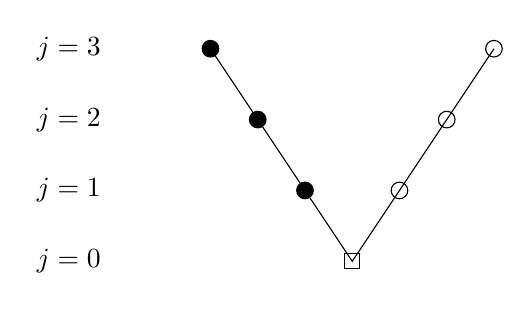
\begin{tikzpicture}[scale=1.2]
  \pgfmathsetmacro\hstep{0.5}
  \pgfmathsetmacro\vstep{0.75}
  \pgfmathsetmacro\ceps{0.08}   % size of square for coarse grid

% grid labels at left
  \node at (-2,3*\vstep) {$j=3$};
  \node at (-2,2*\vstep) {$j=2$};
  \node at (-2,\vstep) {$j=1$};
  \node at (-2,0.0) {$j=0$};

% V-cycle
  \draw[black,thin] (-\hstep,3*\vstep) -- (0.0,2*\vstep) -- (\hstep,\vstep) --  (2*\hstep,0.0)
                    -- (3*\hstep,\vstep) -- (4*\hstep,2*\vstep) -- (5*\hstep,3*\vstep);
  \filldraw (-\hstep,3*\vstep) circle (2.5pt);
  \filldraw (0.0,2*\vstep) circle (2.5pt);
  \filldraw (\hstep,\vstep) circle (2.5pt);
  \draw     (2*\hstep-\ceps,-\ceps) rectangle (2*\hstep+\ceps,+\ceps);
  \draw     (3*\hstep,\vstep) circle (2.5pt);
  \draw     (4*\hstep,2*\vstep) circle (2.5pt);
  \draw     (5*\hstep,3*\vstep) circle (2.5pt);
\end{tikzpicture}

\caption{A V-cycle on a three-level hierarchy ($K=2$) with a down-smoother (solid dots), up-smoother (circles) and coarse-level solver (square).}
\label{fig:vcycle}
\end{figure}

\section{Subset decomposition for the classical obstacle problem} \label{sec:obstacle}

The last section can be read as a quick review, based on the simplest Poisson problem, of a ``classical'' geometric multigrid (GMG) method.  It is not so different from the standard GMG treatments in \cite{Briggsetal2000,Bueler2021,Trottenbergetal2001}, for example.  We have, however, taken a particular FE viewpoint, namely the \emph{subspace decomposition} approach which has been applied both to multilevel and domain decompositions, as pioneered by Xu \cite{Xu1992}.

Classical GMG is, however, not adequate for the main problem in glaciers, namely how the geometry and velocity of a glacier evolves in response to climatic inputs.  First the glaciers problem is (famously) nonlinear, in that the fluid is non-Newtonian, but this is not the leading difficulty.  Rather, regardless of the manner in which momentum (stress) balance is modeled, the boundary condition for the geometry evolution (i.e.~mass conservation) problem arises from an inequality constraint.  Namely that the ice thickness is nonnegative, equivalently that the ice surface elevation is above the bed elevation, a point already made in the Introduction but actually addressed in the next section.  For now we note that the addition of such an inequality constraint generates a nonlinear problem, even if the differential equation is linear.  In this section we modify the GMG subspace decomposition approach to solve a classical \emph{obstacle} problem, which combines an inequality constraint with a linear differential equation.  Switching the differential equation to the nonlinear SIA model in the next section will be comparatively an easy change; one can say that the dominant nonlinearity is already present in the classical obstacle problem here.

We solve the classical obstacle problem by a \emph{constraint decomposition} \cite{Tai2003} method, which modifies the subspace decomposition to allow an inequality constraint.  FIXME

FIXME cite for multigrid obstacle \cite{BrandtCryer1983,Bueler2021,GraeserKornhuber2009,Jouvetetal2013}; cite for subset decomp \cite{Tai2003}


\section{Multigrid solutions of a shallow-ice mass conservation problem} \label{sec:sia}

FIXME cite for glaciers as obstacle problems \cite{Bueler2016,Bueler2020,Calvoetal2002,JouvetBueler2012}

FIXME for 2D domains the coarse mesh construction needs reconsideration

\section{Multigrid solutions of a Glen-Stokes glacier flow} \label{sec:stokes}

FIXME multigrid already used for Blatter-Pattyn model \cite{BrownSmithAhmadia2013} and for hybrid \cite{Jouvetetal2013}; one goal of this section is to make these approaches more understandable

FIXME we use Schur complement \cite{Bueler2021,Elmanetal2014} and compare it to Vanka monolithic smoother \cite{Farrelletal2019}

\small

\bigskip
\bibliography{review}
\bibliographystyle{siam}

\end{document}
